%!TEX root = ../../../memoria.tex
\section{Profile}

	La \uiSiglaAS de profile permite ver y editar información relacionada directamente con el usuario. Esta información está dividida en dos partes: actualización de contraseña y libreta de direcciones.

	\subsection{Actualizar contraseña}

		El formulario de actualización de contraseña permite al usuario cambiar tanto como desee la contraseña que tiene actualmente. Después de todo, el cambio periódico de una contraseña es una medida de seguridad básica \cite{zviran1999password}.
		%The periodic changing ofa password is a basic security measure  

		Como se puede observar en la \refFigura{figure:profile:form:form_update_password}, el formulario de actualización de contraseña cuenta con dos campos obligatorios para el proceso. El primero corresponde al campo de solicitud de contraseña actual (a modo de confirmación de que la persona que está actualizando la contraseña, sea el dueño de la cuenta) y el segundo campo, para ingresar la nueva contraseña. Al apretar el botón de confirmación esta se cambia.

		\begin{figure}[h!]
			\centering
			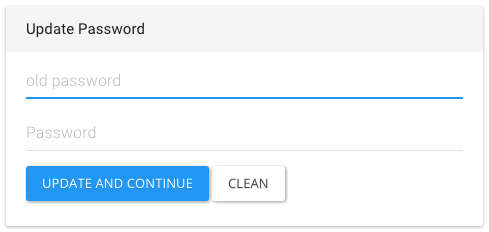
\includegraphics[width=0.5\textwidth]{figuras/profile/form_update_password.png}

			\caption{Formulario de actualización de contraseña.}
			\label{figure:profile:form:form_update_password}
		\end{figure}

		Existen diversas situaciones en donde el formulario notifica sobre errores que se cometen  al momento de llenar el formulario. Por ejemplo, al intentar enviar el formulario sin información ambos campos tienen errores y pueden observarse en la \refFigura{figure:apendice:profile:form:update_password:empty_form_send}.



		\begin{table}[h!]
		    \centering
			\begin{tabular}{ |l|c||l| }
				\hline Campo & Requerido & Restricción \\ \hline
				\multirow{1}{*}{\textit{Current Password}} 	&  \checkmark 					&  Debe ser la contraseña actual.\\ \hline
				\multirow{2}{*}{\textit{Password}} 			&  \multirow{2}{*}{\checkmark}	&  - Debe tener al menos 8 caracteres.\\
															&  								&  - Debe tener al menos un número o símbolo.\\ \hline
			\end{tabular}
		 	\caption{Resumen restricciones formulario edición de contraseña (\refFigura{figure:apendice:profile:form:update_password:empty_form_send}  y \refFigura{figure:apendice:profile:form:update_password:week_password}).}
		    \label{tab:profile:form:restrictions:update_password}
		\end{table}


		Tanto en la \refFigura{figure:apendice:profile:form:update_password:empty_form_send} y en la \refFigura{figure:apendice:profile:form:update_password:week_password} se puede observar que la nueva contraseña no cumple con estos requerimientos.
		Los requerimientos solicitados no responden a ninguna política de seguridad actual. Simplemente se eligieron esos requerimientos para evitar contraseñas aún más débiles que las que se pueden generar.


		Existe un último error, y corresponde simplemente cuando el usuario no logra identificarse correctamente, o lo que es equivalente, la contraseña actual ingresada no es correcta. En la \refFigura{figure:apendice:profile:form:update_password:incorrect_password} puede observarse el mensaje que el formulario entrega en este caso.


		% \subsubsection{Ordenes de compra}

		% 	El backend de las ordenes de compra aún no esta terminado, de momento solo esta el mensaje cuando no hay ninguna orden (\refFigura{figure:profile:orders_empty}).

		% 	\begin{figure}[h!]
		% 	\centering
		% 	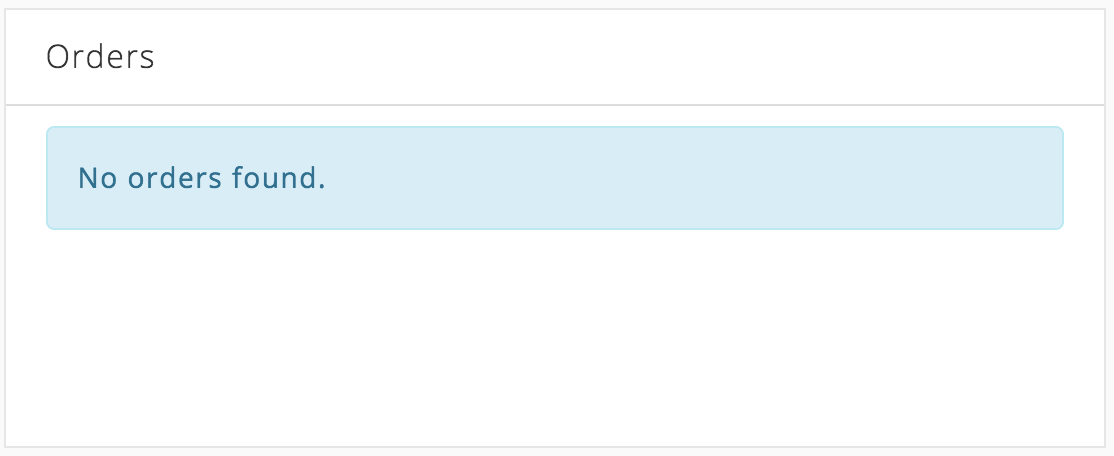
\includegraphics[width=0.5\textwidth]{figuras/profile/orders_empty.png}

		% 	\caption{Vista de ordenes cuando no hay ninguna.}
		% 	\label{figure:profile:orders_empty}
		% \end{figure}



	\subsection{Libreta de direcciones}\label{chapter:solucionimplementada:section:profile:subsection:book_address}

		Corresponde a todas las direcciones que el usuario ha agregado al sistema con el fin de utilizarlas para la recepción del o los productos y de las facturas. Cada uno de los parámetros del formulario para una dirección fue elegido a partir del formulario de direcciones que utiliza \amazonNAME (\refFigura{figure:apendice:address:example:amazon_address}).

		Como buena práctica, se debe utilizar la dirección de \ShippingCOM como dirección \defaultCPT para la dirección de facturación. Los clientes típicamente ordenan productos para la dirección del hogar. Así que por \defaultCPT, se debe utilizar la misma dirección para ambos casos\cite{online_official_smashingmagazine_fundamental_guidelines_checkout_design}.
		%8. Use Shipping Address As Billing Address By Default Link
		% Issue: Most customers order products to their home, so requiring both a billing and shipping address doesn’t make sense.
		% Customers typically order products to their home address. So, by default, you should use the same address for shipping and billing, unless you happen to record data differently for your store.
		Dejando la dirección de facturación por \defaultCPT como la de \ShippingCOM, el proceso de \checkoutCOM tendrá algunos campos menos, haciendo el proceso menos intimidante para los clientes. Los usuarios también disminuyen el riesgo de cometer un error al escribir sus direcciones solo una vez; ellos no se moverán a través del formulario de manera tan rápida y de existir errores, el usuario solo tendrá que resolverlos una vez \cite{online_official_smashingmagazine_fundamental_guidelines_checkout_design}.
		% By defaulting the billing address to the shipping address, your checkout process will have many fewer fields, making it less intimidating for customers. Users also reduce the risk of misspelling their address if they have to enter it only once; they won’t rush through the form as quickly, and if there are errors, the customer will have to fix them only once.

		Teniendo en consideración estos detalles, se desarrolla el formulario que se observa en la \refFigura{figure:address:form:add_new_address}.

		\begin{figure}[h!]
			\centering
			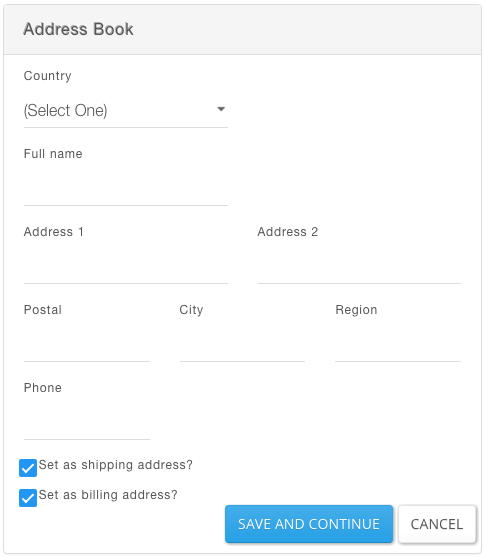
\includegraphics[width=0.7\textwidth]{figuras/address/form/add_new_address.png}
			\caption{Formulario para agregar una nueva dirección.}
			\label{figure:address:form:add_new_address}
		\end{figure}

		Este formulario cuenta con las restricciones descritas en la \reftabla{tab:profile:form:restrictions:address}, y por lo tanto muestra mensaje de error según corresponda.
		%TODO : Agregar figuras del formulario con diferentes tipos de errores en el apendice y referenciarlos acá

		\begin{table}[H]
		    \centering
			\begin{tabular}{ |l|c||l| }
				\hline Campo & Requerido & Restricción \\ \hline
				\multirow{1}{*}{\textit{Country}} 			&  \checkmark 	&  Debe ser una de las alternativas.\\ \hline
				\multirow{1}{*}{\textit{Full Name}} 		&  \checkmark	& \\ \hline
				\multirow{1}{*}{\textit{Address 1}} 		&  \checkmark	& \\ \hline
				\multirow{1}{*}{\textit{Address 2}} 		&  				& \\ \hline
				\multirow{1}{*}{\textit{Postal}} 			&  \checkmark	& \\ \hline
				\multirow{1}{*}{\textit{City}} 				&  \checkmark	& \\ \hline
				\multirow{1}{*}{\textit{Region}} 			&  \checkmark	& Para ciertos países, existen alternativas definidas.\\ \hline
				\multirow{1}{*}{\textit{Phone}} 			&  \checkmark	& \\ \hline
				\multirow{1}{*}{\textit{Shipping address}} 	&  \checkmark	& Boolean. \\ \hline
				\multirow{1}{*}{\textit{billing address}} 	&  \checkmark	& Boolean. \\ \hline
				%\multirow{1}{*}{\textit{comercial address}} &  \checkmark	& Boolean. \\ \hline
			\end{tabular}
		 	\caption{Resumen restricciones formulario para libreta de direcciones.}
		    \label{tab:profile:form:restrictions:address}
		\end{table}

		Notar que en la parte superior de la \refFigura{figure:address:form:add_new_address} está el botón que permite ingresar nuevas direcciones. Cada una de estas nuevas direcciones es agregada a la lista que aparece en la \refFigura{figure:address:form:list_address}, lugar en donde pueden ser editadas y eliminadas de acuerdo a las necesidades del cliente. En caso de editar alguna dirección, esta debe cumplir las mismas restricciones impuestas para el caso de la creación de una dirección (\reftabla{tab:profile:form:restrictions:address}).

		\begin{figure}[H]
			\centering
			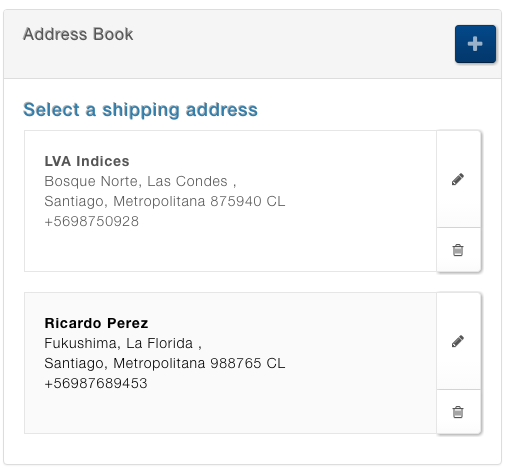
\includegraphics[width=0.7\textwidth]{figuras/address/form/list_address.png}
			\caption{Lista con todas las direcciones configuradas del usuario. Cada una de estas puede ser editada o eliminada con los botones que se encuentran en el costado derecho.}
			\label{figure:address:form:list_address}
		\end{figure}

		Es importante agregar que en la situación en que el usuario no tenga configurada ninguna dirección, aparecerá por \defaultCPT el formulario de creación. Esto se observa en la \refFigura{figure:address:form:add_first_address}.

		\begin{figure}[H]
			\centering
			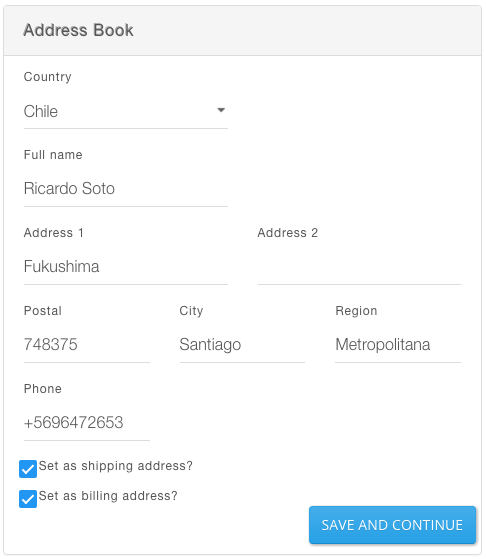
\includegraphics[width=0.7\textwidth]{figuras/address/form/add_first_address.png}
			\caption{Formulario para agregar una nueva dirección, aparece en caso de no existir configurada ninguna previa. Notar que no existe un botón para cancelar dado que en este contexto no tiene sentido.}
			\label{figure:address:form:add_first_address}
		\end{figure}




